\begin{frame}{Calcul des points cibles}
    \begin{columns}
        \begin{column}{0.48\textwidth}
            \textbf{Problème : Point cible unique}
            \begin{figure}[h!]
                \centering
                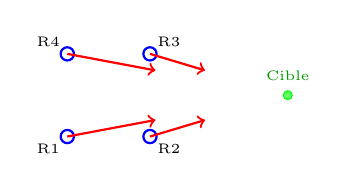
\begin{tikzpicture}[scale=0.7, every node/.style={font=\tiny}]
                    \usetikzlibrary{calc}
                    % Robots (carré, cercles blancs)
                    \filldraw[fill=white,draw=blue,thick] (0,0) circle (0.12) node[below left=-1pt] {R1};
                    \filldraw[fill=white,draw=blue,thick] (1.5,0) circle (0.12) node[below right=-1pt] {R2};
                    \filldraw[fill=white,draw=blue,thick] (1.5,1.5) circle (0.12) node[above right=-1pt] {R3};
                    \filldraw[fill=white,draw=blue,thick] (0,1.5) circle (0.12) node[above left=-1pt] {R4};
                    
                    % Point cible global
                    \coordinate (cible) at (4,0.75);
                    \filldraw[fill=green!60,draw=green] (cible) circle (0.08);
                    \node[green!60!black] at (4,1.1) {\tiny Cible};
                    
                    % Vecteurs de vitesse vers le point cible global
                    \draw[->,thick,red] (0,0) -- ($(0,0)!0.4!(cible)$);
                    \draw[->,thick,red] (1.5,0) -- ($(1.5,0)!0.4!(cible)$);
                    \draw[->,thick,red] (1.5,1.5) -- ($(1.5,1.5)!0.4!(cible)$);
                    \draw[->,thick,red] (0,1.5) -- ($(0,1.5)!0.4!(cible)$);
                \end{tikzpicture}
            \end{figure}
            
            \textbf{Conséquences :}
            \begin{itemize}
                \item Risque de collisions
                \item Perte de formation
            \end{itemize}
        \end{column}
        \begin{column}{0.48\textwidth}
            \textbf{Solution : Points cibles individuels}
            \begin{figure}[h!]
                \centering
                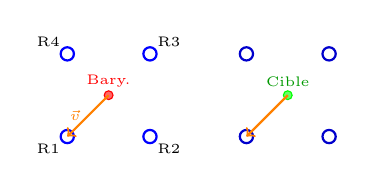
\begin{tikzpicture}[scale=0.7, every node/.style={font=\tiny}]
                    % Robots initiaux
                    \filldraw[fill=white,draw=blue,thick] (0,0) circle (0.12) node[below left=-1pt] {R1};
                    \filldraw[fill=white,draw=blue,thick] (1.5,0) circle (0.12) node[below right=-1pt] {R2};
                    \filldraw[fill=white,draw=blue,thick] (1.5,1.5) circle (0.12) node[above right=-1pt] {R3};
                    \filldraw[fill=white,draw=blue,thick] (0,1.5) circle (0.12) node[above left=-1pt] {R4};
                    % Barycentre initial
                    \filldraw[fill=red!60,draw=red] (0.75,0.75) circle (0.08);
                    \node[red] at (0.75,1) {\tiny Bary.};
                    
                    % Point cible global
                    \filldraw[fill=green!60,draw=green] (4,0.75) circle (0.08);
                    \node[green!60!black] at (4,1) {\tiny Cible};
                    
                    % Points cibles individuels
                    \filldraw[fill=white,draw=blue!80!black,thick] (3.25,0) circle (0.12);
                    \filldraw[fill=white,draw=blue!80!black,thick] (4.75,0) circle (0.12);
                    \filldraw[fill=white,draw=blue!80!black,thick] (4.75,1.5) circle (0.12);
                    \filldraw[fill=white,draw=blue!80!black,thick] (3.25,1.5) circle (0.12);
                    
                    % Vecteur relatif exemple
                    \draw[->,thick,orange] (0.75,0.75) -- (0,0) node[midway,left=-1pt,orange] {\tiny $\vec{v}$};
                    \draw[->,thick,orange] (4,0.75) -- (3.25,0);
                \end{tikzpicture}
            \end{figure}
            
            \begin{equation}
                \mathbf{p}_r^i = \mathbf{p}_\text{goal} + (\mathbf{p}_i^\text{init} - \mathbf{p}_\text{bary}^\text{init})
            \end{equation}
        \end{column}
    \end{columns}
\end{frame}

\begin{frame}{Adaptation du coefficient $c_1^\gamma$}
    \textbf{Rappel - Terme de navigation :}
    \begin{equation}
        \mathbf{u}_i^{\gamma} = -c_{1,\gamma}(\mathbf{p}_i - \mathbf{p}_r)
    \end{equation}
    
    \begin{columns}
        \begin{column}{0.5\textwidth}
            \textbf{Objectif :}
            \begin{itemize}
                \item Adapter dynamiquement l'attraction vers la cible
            \end{itemize}
            
            \vspace{0.5cm}
            \textbf{Principe :}
            \begin{itemize}
                \item Surveillance continue des ratios de distance
                \item Réduction progressive selon la gravité
            \end{itemize}
        \end{column}
        \begin{column}{0.5\textwidth}
            \textbf{Trois niveaux d'adaptation :}
            \begin{enumerate}
                \item \textcolor{red}{Cas extrêmes} : $c_1^\gamma \approx 0$
                \item \textcolor{green}{Formation correcte} : $c_1^\gamma = 0.2$
                \item \textcolor{orange}{Formation imparfaite} : réduction progressive
            \end{enumerate}
                        
        \end{column}
    \end{columns}
\end{frame}
